\hypertarget{index_req_sec}{}\section{Requirements}\label{index_req_sec}

\begin{DoxyItemize}
\item xerces-\/c
\item cppunit
\item log4cxx
\end{DoxyItemize}

Using linux is advised!\hypertarget{index_args_sec}{}\section{Running Arguments}\label{index_args_sec}

\begin{DoxyCode}
export OMP\_NUM\_THREADS=8
./MolSim filename
\end{DoxyCode}
 Run the simulation with configurations defined in \textquotesingle{}filename\textquotesingle{}. Set the environment variable {\bfseries O\+M\+P\+\_\+\+N\+U\+M\+\_\+\+T\+H\+R\+E\+A\+DS} to define the number of threads used.


\begin{DoxyCode}
./MolSim -test [TestSuite]
\end{DoxyCode}
 Run the testsuites. A specific suite can be passed. Otherwise all suites will be processed.\hypertarget{index_cfile_ssec}{}\subsection{Configuration File}\label{index_cfile_ssec}
Configuration files are xml file which specify needed setting. These start with a {\bfseries setting}-\/element which contains follwing property-\/elements\+:
\begin{DoxyItemize}
\item {\bfseries outputname} -\/ Base name of the output files
\item {\bfseries endfile} -\/ Optional\+: save last particle states into a new xml input-\/file
\item {\bfseries inputfiles} -\/ File containing information to create particles
\item {\bfseries frequency} -\/ Write frequency of the output files
\item {\bfseries profile\+File} -\/ Optional\+: Write profile of y-\/velocity into this file
\item {\bfseries profile\+BucketsX} -\/ Optional\+: Number of divisions in x-\/direction to profile y-\/velocity
\item {\bfseries delta\+\_\+t} -\/ The time step between iterations
\item {\bfseries t\+\_\+end} -\/ Time to simulate
\item {\bfseries sigma} -\/ Sigma for Lennard-\/\+Jones calculation
\item {\bfseries epsilon} -\/ Epsilon for Lennard-\/\+Jones calculation
\item {\bfseries b\+\_\+factor} -\/ Factor for Maxwell-\/\+Boltzmann Distribution
\item {\bfseries g\+\_\+grav\+\_\+x} -\/ Acceleration due to gravity in x-\/direction
\item {\bfseries g\+\_\+grav\+\_\+y} -\/ Acceleration due to gravity in y-\/direction
\item {\bfseries g\+\_\+grav\+\_\+z} -\/ Acceleration due to gravity in z-\/direction
\item {\bfseries domainX} -\/ x-\/\+Dimension of domain
\item {\bfseries domainY} -\/ y-\/\+Dimension of domain
\item {\bfseries domainZ} -\/ z-\/\+Dimension of domain
\item {\bfseries r\+\_\+cutoff} -\/ Maximum cutoff radius
\item {\bfseries bc\+\_\+left} -\/ Boundary condition at x=0\+: 1 is reflecting boundaries, 2 is periodic boundaries, else it is an outflow
\item {\bfseries bc\+\_\+lower} -\/ Boundary condition at y=0\+: 1 is reflecting boundaries, 2 is periodic boundaries, else it is an outflow
\item {\bfseries bc\+\_\+upper} -\/ Boundary condition at y=domainY\+: 1 is reflecting boundaries, 2 is periodic boundaries, else it is an outflow
\item {\bfseries bc\+\_\+right} -\/ Boundary condition at x=domainX\+: 1 is reflecting boundaries, 2 is periodic boundaries, else it is an outflow
\item {\bfseries bc\+\_\+front} -\/ Boundary condition at z=0\+: 1 is reflecting boundaries, 2 is periodic boundaries, else it is an outflow
\item {\bfseries bc\+\_\+back} -\/ Boundary condition at z=domainZ\+: 1 is reflecting boundaries, 2 is periodic boundaries, else it is an outflow
\item {\bfseries thermostat} -\/ Optional\+: Defines a thermostat that keeps the simulation at given temperature. This will override {\bfseries b\+\_\+factor}!
\begin{DoxyItemize}
\item {\bfseries initial} -\/ inital temperature
\item {\bfseries timestep} -\/ number of timesteps after which the thermostat is applied
\item {\bfseries ignoreY} -\/ Optional\+: true if the thermostat does not affect the y-\/component of the velocity
\item {\bfseries heating} -\/ Optional\+: defines a temperature change over time
\begin{DoxyItemize}
\item {\bfseries target} -\/ target temperature
\item {\bfseries temperature\+\_\+step} -\/ step size in which the temperature should be changed
\item {\bfseries timestep} -\/ number of timesteps after which the temperature is changed
\end{DoxyItemize}
\end{DoxyItemize}
\end{DoxyItemize}

Example file\+: setting.\+xml\hypertarget{index_ifile_ssec}{}\subsection{Input File}\label{index_ifile_ssec}
Input files are xml files which specify the particles in given simulation. These start with a particle\+\_\+input-\/element which can contain following elements with subelements\+:
\begin{DoxyItemize}
\item {\bfseries types\+\_\+input} -\/ Defines the properties of a type
\begin{DoxyItemize}
\item {\bfseries id} -\/ The unique identifier of the type
\item {\bfseries mass} -\/ The mass of a particle of this type
\item {\bfseries sigma} -\/ The sigma used for the Lennard-\/\+Jones formula
\item {\bfseries epsilon} -\/ The epsilon used for the Lennard-\/\+Jones formula
\item {\bfseries fixed} -\/ Optional\+: true if particle cannot be moved
\item {\bfseries Rtrunc\+LJ} -\/ Optional\+: distance at which the Lennard-\/\+Jones force calculation should be truncated, if not specified, it will be set to Rcutoff
\end{DoxyItemize}
\item {\bfseries single\+\_\+input} -\/ Create a single particle
\begin{DoxyItemize}
\item {\bfseries coord} -\/ Position of particle
\item {\bfseries force} -\/ Optional\+: Current force enacting on the particle
\item {\bfseries velocity} -\/ Initial velocity of the partilce
\item {\bfseries type} -\/ id of the type of the particle
\end{DoxyItemize}
\item {\bfseries cuboid\+\_\+input} -\/ Create a cuboid of particles
\begin{DoxyItemize}
\item {\bfseries coord} -\/ Position of lower left front corner of the cuboid
\item {\bfseries dimension} -\/ Number of particles in each dimension
\item {\bfseries mesh} -\/ Spacing between each particle
\item {\bfseries velocity} -\/ Initial mean velocity of each particle
\item {\bfseries type} -\/ id of the type of the particle
\end{DoxyItemize}
\item {\bfseries sphere\+\_\+input} -\/ Create a sphere of particles
\begin{DoxyItemize}
\item {\bfseries coord} -\/ Center of the sphere
\item {\bfseries radius} -\/ Number of particles as radius
\item {\bfseries mesh} -\/ Spacing between each particle
\item {\bfseries velocity} -\/ Initial mean velocity of each particle
\item {\bfseries type} -\/ id of the type of the particle
\end{DoxyItemize}
\item {\bfseries membrane\+\_\+input} -\/ Create a membrane of particles
\begin{DoxyItemize}
\item {\bfseries stiffness} -\/ stiffness k of the membrane
\item {\bfseries r\+\_\+zero} -\/ average bond length of a molecule pair
\item {\bfseries force} -\/ Optional\+: force which acts on certain molecules
\item {\bfseries t\+\_\+end\+\_\+force} -\/ Optional\+: time when the optional force stops to act
\item {\bfseries coord\+\_\+force} -\/ mesh coordinates of the particles where the force acts
\item {\bfseries coord} -\/ Position of lower left front corner of the cuboid
\item {\bfseries dimension} -\/ Number of particles in each dimension
\item {\bfseries mesh} -\/ Spacing between each particle
\item {\bfseries velocity} -\/ Initial mean velocity of each particle
\item {\bfseries type} -\/ id of the type of the particle
\end{DoxyItemize}
\end{DoxyItemize}

Example files\+: eingabe-\/cuboid.\+xml\hypertarget{index_perf_sec}{}\section{Performance}\label{index_perf_sec}
The following graph compares the runtime of Linked cells algorithm to the use of a non-\/optimized algorithm. The tests were runned on 1000, 2000, 4000 and 8000 particles for 5s with a time step of 0.\+0005s.   
\begin{DoxyImage}
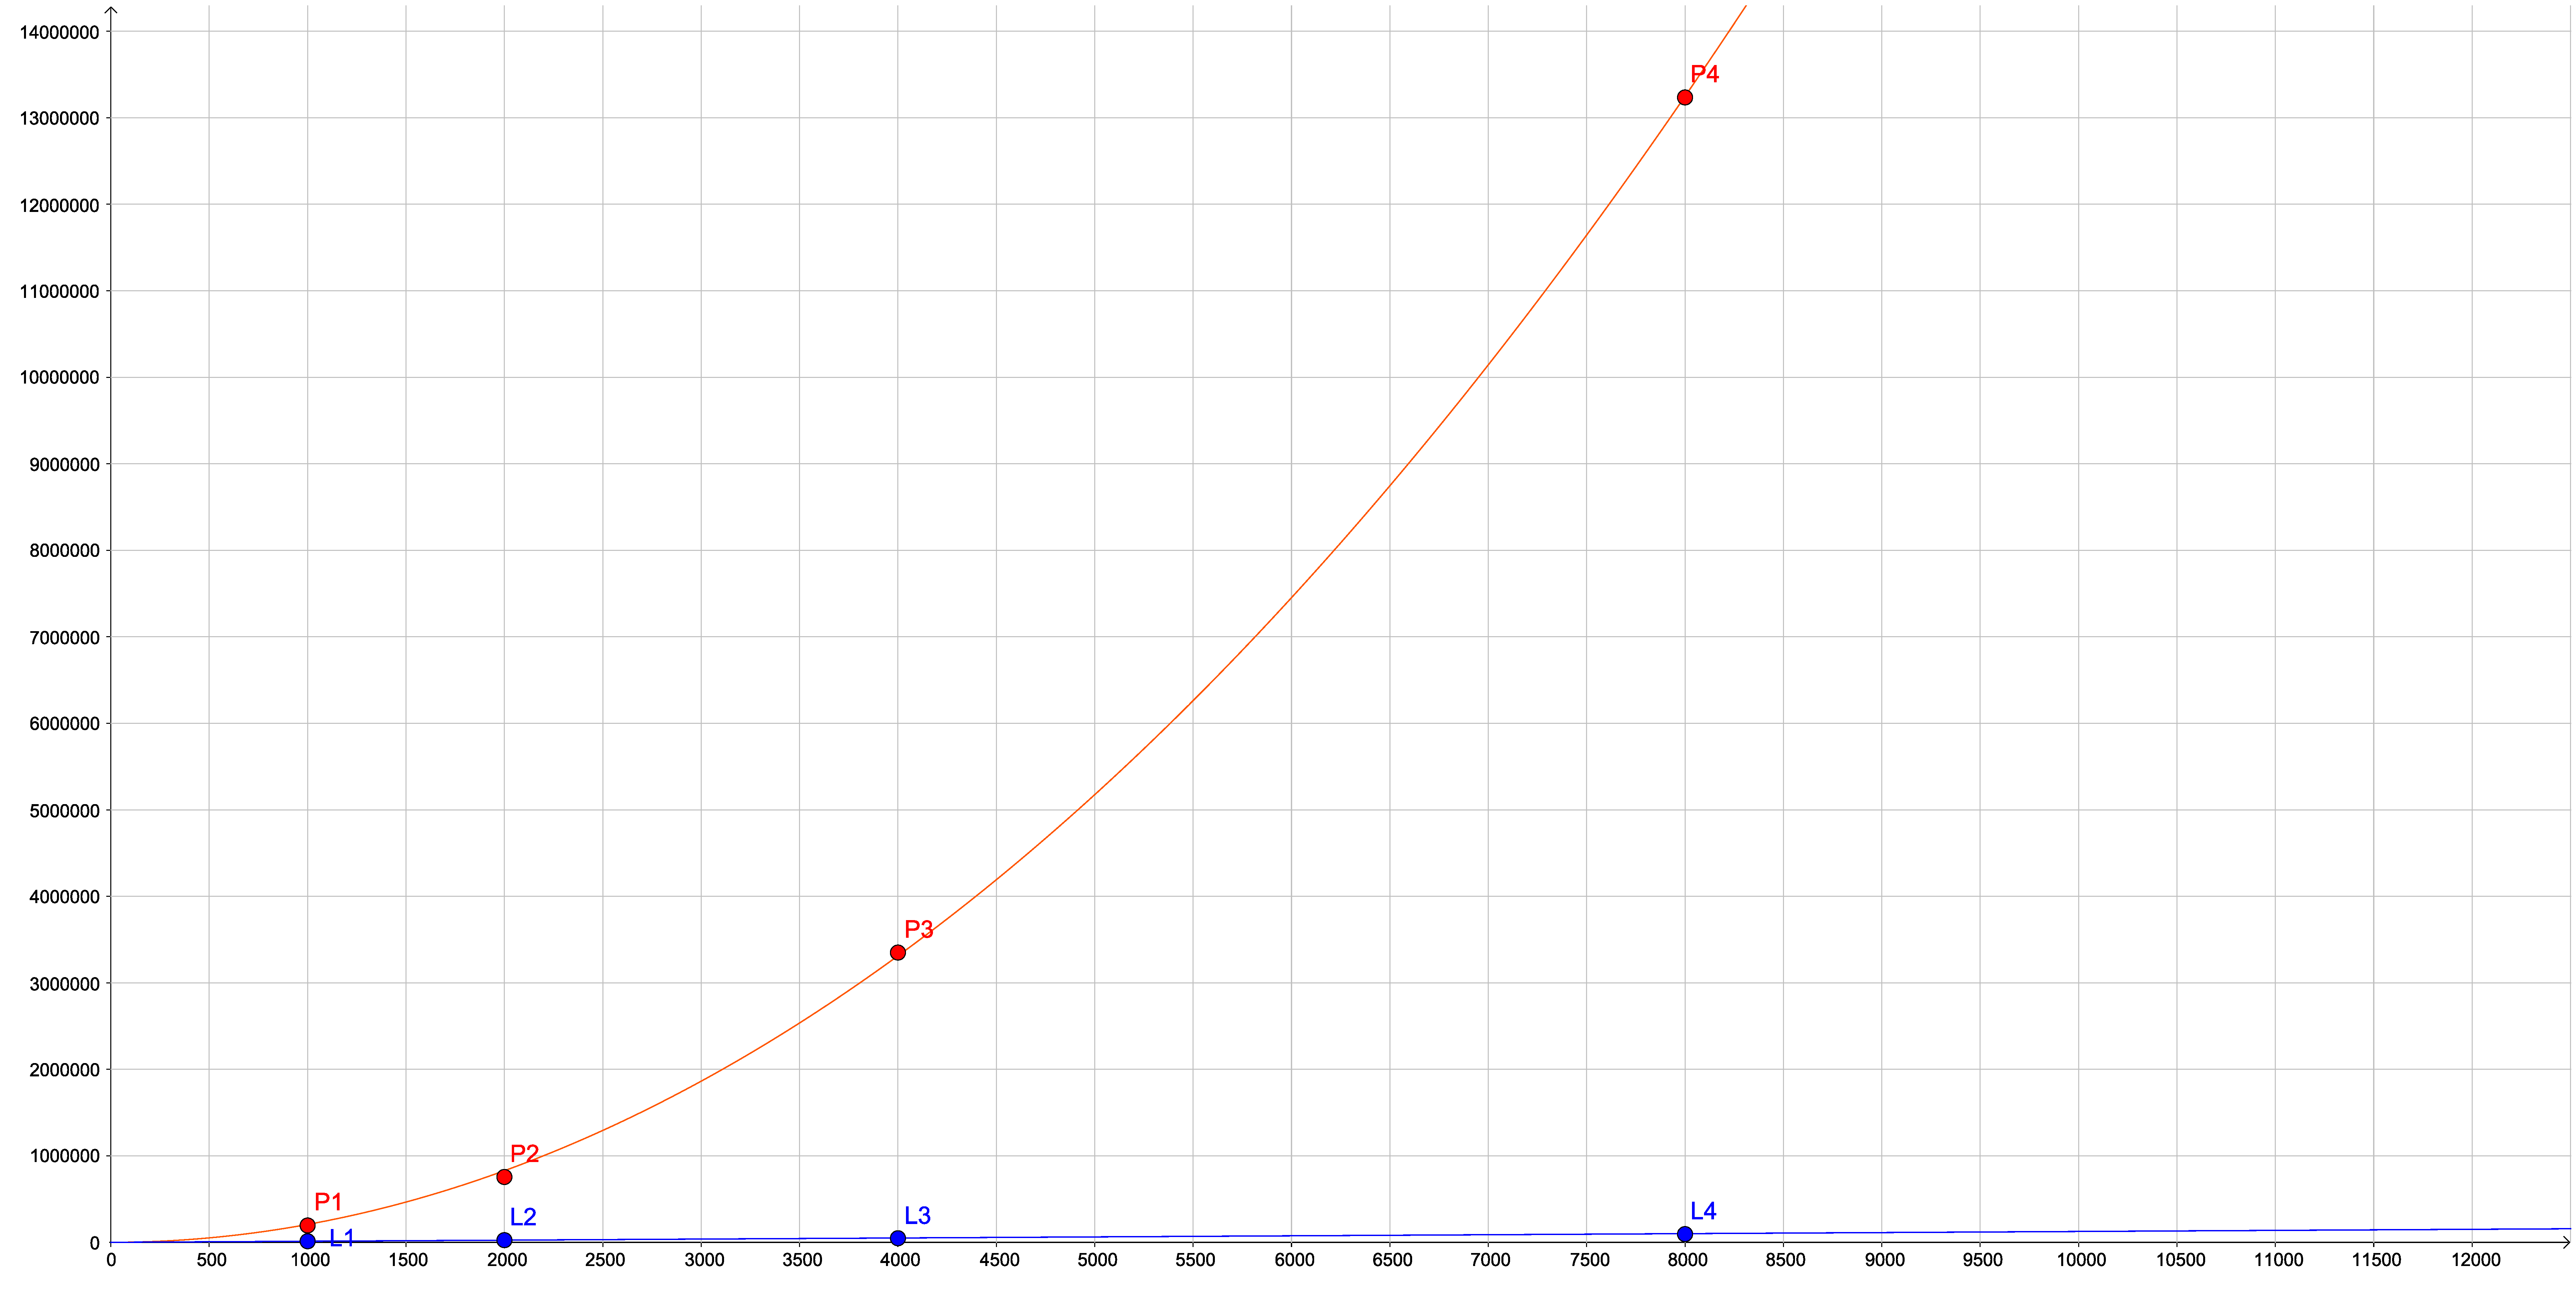
\includegraphics[width=40cm]{test}
\caption{Performance test}
\end{DoxyImage}
\hypertarget{index_thread_sec}{}\section{Parallelization}\label{index_thread_sec}
The following graph compares the Molecule-\/\+Updates per Second depending on the number of threads used. The configuration file used was setting-\/liquid.\+xml   
\begin{DoxyImage}
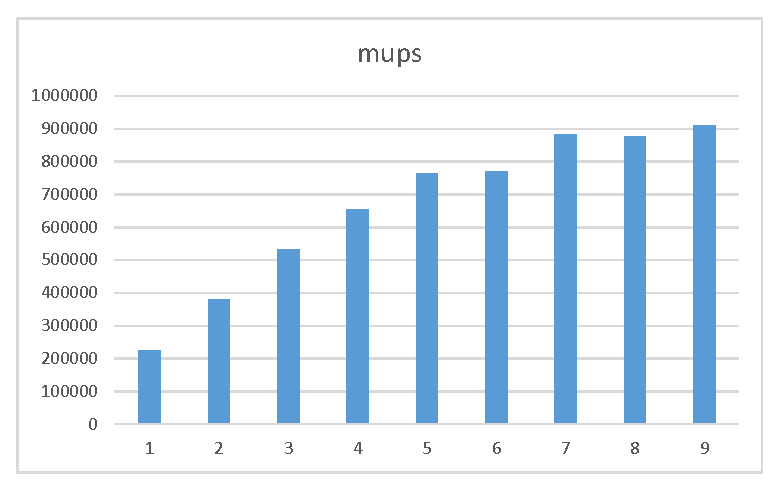
\includegraphics[width=40cm]{mups}
\caption{Performance test}
\end{DoxyImage}
 